\documentclass{finalreport}
\usepackage[utf8]{inputenc}

\DeclareSourcemap{
 \maps[datatype=bibtex]{
   \map{
     \step[fieldsource=url,
       match=\regexp{\\_},
       replace=\regexp{_}]
   }
 }
}

\addbibresource{citations.bib}


%%% Template Usage
% 1. Go to "All Projects" and make a copy in Overleaf,
% or download the source to modify locally.
% 2. Fill in your name
% 3. Set the reportdate to Monday of the current week


\title{Using Toy Networks to Model Disruptions in Science Networks}
\author{Edris Qarghah}

\DTMsavedate{startdate}{2020-07-07}
\DTMsavedate{enddate}{2020-09-15}
\date{\DTMusedate{startdate}-\DTMusedate{enddate}}



\makenoidxglossaries

\newglossaryentry{esnet}{name={ESnet},
 description={A high-bandwidth network, managed by the Lawrence Berkeley National Laboratory, that connects scientists at national laboratories, universities and other research institutions within the US}}
\newglossaryentry{bridge}{name={bridge-connected},
 description={A subgraph connected to the rest of the graph by a single edge (a bridge\cite{bridge}, which would become a separate \gls{component} if that edge were removed}}
\newglossaryentry{betweenness}{name={Betweenness Centrality},
 description={The centrality\cite{centrality} of an vertex in a graph can be defined in many ways. Betweenness centrality does so by calculating the number of paths along which a given node is essential (i.e., without the node, there would no longer be a connection between two other nodes)}}
\newglossaryentry{boundary}{name={boundary\cite{boundary}},
 plural={boundaries},
 description={A \gls{node} or set of nodes that are between two subgraphs}}
\newglossaryentry{hub}{name={hub\cite{hub}},
 description={A \gls{node} with significantly more links than average}}
\newglossaryentry{degree}{name={degree\cite{degree}},
 description={The number of edges connected to a node.}}
\newglossaryentry{anomaly}{name={anomaly detection},
 description={The identification of events on the network that are outside the norm}}
\newglossaryentry{connected}{name={connected\cite{connectivity}},
 description={A graph is said to be connected, if all nodes can be reached from all other nodes.}}
\newglossaryentry{kconnected}{name={$k$-connected\cite{connectivity}},
 description={A graph is said to be $k$-connected, if removing $k$ edges somewhere in the graph would result in the graph no longer being \gls{connected}}}
\newglossaryentry{component}{name={component\cite{connectivity}},
 description={A cohesive subgraph containing any number of connected nodes. A \gls{connected} graph has one component (the entire graph), but a \gls{kconnected} graph would break into more, smaller components if particular sets of $k$ edges were cut}}
\newglossaryentry{endpoint}{name={endpoint},
 description={The devices that serve as the source or destination of a transmission along the network. While any device could serve as an endpoint, the only endpoints we are concerned with (as they are the only ones regarding which we have data), are \glspl{psnode}}}
\newglossaryentry{hop}{name={hop},
 description={Each step along the network from one device to the next (and sometimes within the same device). The hop is usually documented via \gls{trace} and is identified by the \gls{ip} of the device the hop arrives at}}
\newglossaryentry{ipadd}{name={IP address\cite{ip}},
 description={An Internet Protocol (IP) address is a 32-bit (IPv4) or 128-bit (IPv6) number that identifies a device on a network}}
\newglossaryentry{latency}{name={latency},
 plural={latencies},
 description={The amount of time it takes for one bit of data to travel along a network from one \gls{endpoint} to another}}
\newglossaryentry{tomography}{name={network tomography},
 description={The study of the shape, state and other characteristics of a network using only data gathered from limited set of \glspl{endpoint}}}
\newglossaryentry{node}{name={node},
 description={A device connected to the network which may serve as a \gls{hop} between two \glspl{endpoint}}}
\newglossaryentry{packetloss}{name={packet loss},
 description={The percentage of packets of data that failed to reach their destination. The \gls{tcp} identifies and re-transmits lost packets, but this can slow transmission down to a trickle}}
\newglossaryentry{delay}{name={one-way delay},
 description={The amount of time it takes for data to be transmitted from a source \gls{ps} node to a destination. This is measured by the difference in clock measurements between \glspl{endpoint}}}
\newglossaryentry{perfsonar}{name={perfSONAR\cite{perfsonar}},
 description={Short for performance Service-Oriented Network monitoring ARchitecture, it is a network measurement toolkit designed to provide federated coverage of paths and help to establish end-to-end usage expectations}}
\newglossaryentry{psnode}{name={perfSONAR (PS) node},
 description={Network \glspl{endpoint} equipped with \gls{perfsonar} that send regular communications to one another in order to collect network measurements (i.e., \gls{packetloss}, \gls{latency} and \gls{owd})}}
\newglossaryentry{trace}{name={traceroute},
 description={Data collected about the \glspl{hop} between two \glspl{endpoint}}}

\newacronym{lhc}{LHC}{Large Hadron Collider\cite{lhc}}
\newacronym{owd}{OWD}{\gls{delay}}
\newacronym{ps}{PS}{\gls{perfsonar}}
\newacronym{tcp}{TCP}{Transmission Control Protocol\cite{tcp}}
\newacronym{ip}{IP}{Internet Protocol, though usually synechdoche for \gls{ipadd}}

\begin{document}

\maketitle

\newpage

\section{Abstract}

Tools exist for monitoring networks, but they often rely on measurements taken from a finite number of endpoints on the periphery of the network. These measurements enable the identification of network disruptions, but do not provide direct information on the status of individual connections on the network, making it difficult to pinpoint the location of those disruptions.

In this paper an approach is discussed for creating toy networks, adjusting them to resemble real network distributions and using them to model approaches to network tomography. We also discuss how to adapt these strategies for use with a real network by creating a representation of that network that is analogous to our toy model.

\section*{Introduction}

The \gls{lhc} at CERN\cite{cern} produces exabytes of data that is disseminated to high-energy physics labs around the world for analysis. The network that supports this transmission, which includes \gls{esnet}\cite{esnet} in the United States, is decentralized and consists of approximately $6,000$ individual \glspl{node}\footnote{A survey we conducted of \glspl{trace} from 7/7/2020 to 7/14/2020 found $5968$ unique \glspl{node}.}.

To monitor the activity on the network, certain \glspl{endpoint} are configured as \glspl{psnode}\cite{perfsonar} (around $420$ of them\footnote{The aforementioned survey found $423$ \gls{ps} nodes.}). These regularly transmit data to one another\footnote{The aforementioned survey found \gls{trace} between $24,503$ pairs of \gls{ps} nodes.} and record characteristics of those transmissions, such as \gls{owd}, \gls{packetloss} and \gls{latency}. 

With this limited visibility, if there is a disruption somewhere along the network, it can be hard to pin down where the problem is, potentially leaving entire regions of researchers with slow or limited access to other regions for months at a time.


\subsection*{Identifying Network Disruptions}

This paper represents work toward the goal of developing better methods of determining the source of disruptions on the network used by the high-energy physics community. To address this, we need to:

\begin{itemize}
	\item Identify that there \textit{is} an issue. 
	\begin{itemize}
		\item This is done via \textbf{\gls{anomaly}}, the identification of events that are outside the norm. In our case, this would mean looking at \gls{packetloss}, \gls{owd} and other metrics to see whether any abnormalities may indicate there is a problem that needs to be addressed.
	\end{itemize}
	\item Identify \textit{where} the issue is occurring. 
	\begin{itemize}
		\item To do this, we need to have an understanding of the topology of the network, which is achieved via the use of \textbf{\gls{tomography}}, which is the study of the shape, state and other characteristics of a network using only data gathered from limited set of \glspl{endpoint} (i.e., \glspl{psnode}).
	\end{itemize}
	
\end{itemize}

\noindent In this paper, we are concerned with the latter problem, which we approached in three steps:

\begin{enumerate}
	\item We created a toy network to use as a model.
	\item We developed \gls{tomography} strategies using our toy model.
	\item We created a representation of the real network that mirrors our toy model, so that tools/strategies can be adapted for use with real data.
\end{enumerate}

\section{Toy Network}

\subsection{Motivation}

We have limited visibility into the real network we are working with, as we only have the data collected by \gls{ps} nodes. Such data is incomplete, complicated and messy, so it is not ideal for testing ideas regarding network structure or determining causal relationships in network phenomena. Real data is subject to change for reasons that are sometimes unknowable and often completely outside our control.

This is what motivated the construction of a toy network, one where we could define all nodes and their connections. With such a model, we can make changes, observe the impact on various facets of the network and be certain this impact was caused by our changes. The \gls{tomography} strategies we develop in this controlled environment can then by adapted for use with the real network.

\subsection{Initial Parameters}

It is impractical to create a toy network on the same scale and with the same level of detail as the real one, so we started with the following parameters:

\begin{itemize}
	\item The network consisted of 100 \glspl{node}.
	\item 10 random nodes were selected to ``host" \gls{perfsonar}.
    \item Each node was a coordinate on the $x,y$ plane.
	\item Each node had a random number of connections (up to 4) to its nearest neighbors.
	\item The ``\gls{latency}" for each link was their geometric distance.
\end{itemize}

\begin{figure}[!ht]
\centering
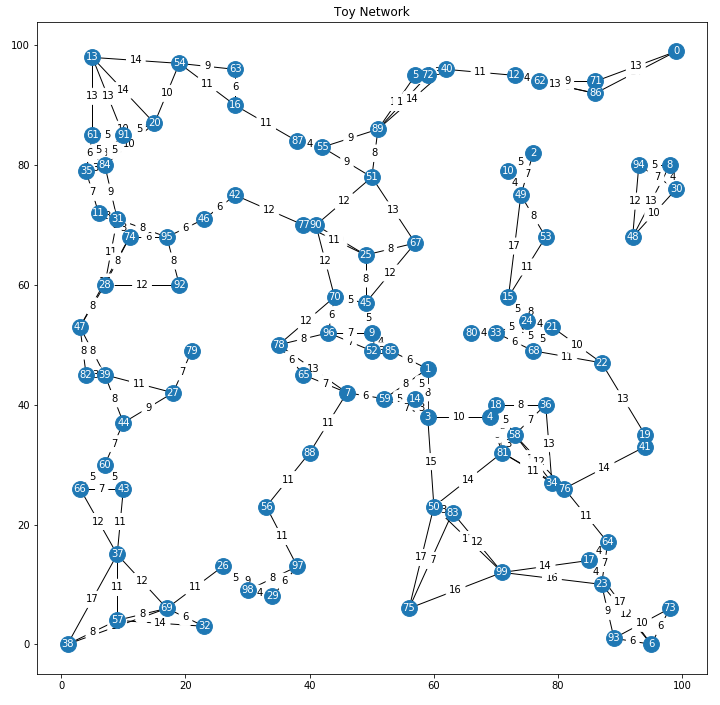
\includegraphics[width=.8\linewidth]{week_1/Network_416b9f8671a64f04a87bbb59c431dc28.png}
\caption{Our first networks had no guarantee of being \gls{connected}, as seen by nodes 94, 8, 48 and 30.}
\end{figure}

\noindent There were some issues with such a na{\"i}ve approach:

\begin{itemize}
    \item There were no long edges (we know this doesn't resemble reality, even without exploring real data, because of transatlantic cables\cite{transatlantic}).
    \item There was no guarantee that all \glspl{component} would be \gls{connected} (for a cluster of nodes, the nearest neighbor to all those nodes may only be within that cluster).
    \item The toy network was not grounded in any information about the real world (i.e., it may not resemble the real network at all, in which case it wouldn't be a very good proxy).
    \item The ``\glspl{psnode}" were indistinguishable from others and had no additional functionality.
\end{itemize}


\subsection*{Incremental Improvements}

As we developed our toy network, we made a wide variety of incremental improvements. The list below highlights changes in roughly chronological order.

\begin{itemize}
    \item We created \gls{hub} nodes that served as a backbone for the network, which were randomly placed in quadrants and quadrants within those quadrants, recursively (it can be configured to any number of layers deep, though we ultimately settled on 5). These hub nodes were connected by edges to the hub nodes within their respective sub-quadrants, ensuring that there were some longer edges and some structure to the network.
    \item We made sure that the network was \gls{kconnected} ($k$ could be configured, though we used $1$-connected), which is to say that there is at least one \gls{component} that could be separated from the rest of the network by cutting $k$ edges.
    \item We colored special nodes (i.e., \gls{hub} and \gls{ps} nodes).
    \item We found the shortest paths between \gls{ps} nodes, using the Euclidean distances between the nodes along the path.
    \item We gave each edge a \gls{packetloss} (and displayed it) based on a distribution pulled from \hyperref[kibana]{Kibana}, but made the mistake of applying the distribution to individual edges and not entire paths.
\end{itemize}

\begin{figure}[!ht]
\centering
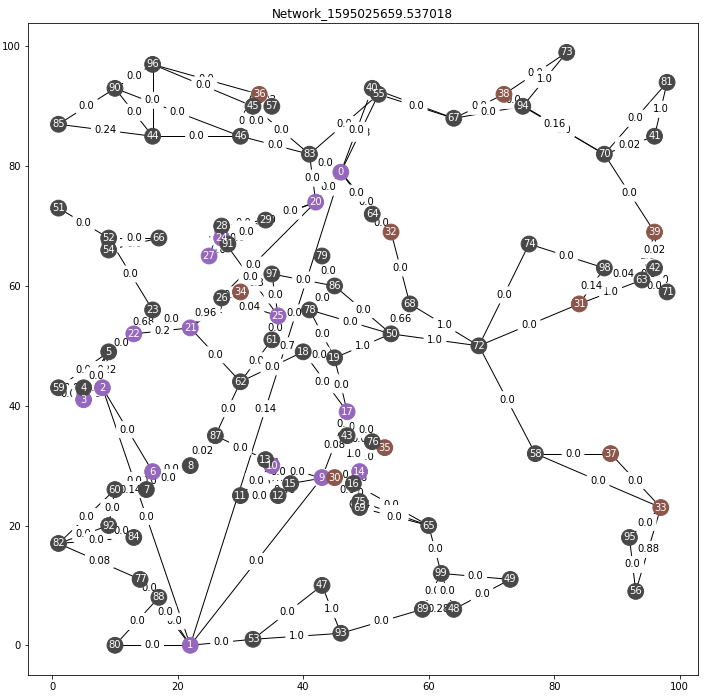
\includegraphics[width=.8\linewidth]{week_2/NetworkZero.png}
\caption{\Gls{hub} (lilac) and \gls{ps} nodes (brown) are colored and there are no unconnected \glspl{component}, but there are components without \gls{ps} nodes (which would never have been seen/traversed on a real network) and the \gls{packetloss} along the edges proved unrealistic.}
\end{figure}

\begin{itemize}
	\item Ensured that all \gls{degree} $1$ nodes are \gls{ps} nodes (if a node is only connected to the network by a single edge, then the only way that node would ever be seen is if that node is itself a \gls{ps} node), but this didn't account for components that didn't contain a \gls{ps} node.
	\item Made sure that all \gls{bridge} components (i.e., \glspl{component} that could be separated from the rest of the network by removing a single edge) have at least \gls{ps} node (otherwise there would be no reason to ever traverse this component).
	\item Used low \gls{betweenness} (roughly a measure of how many paths would be disrupted if a node is removed) as a \gls{ps} selection criteria to ensure that \gls{boundary} nodes (ones connecting a \gls{component} to the rest of the network) are not selected.
	\item Distributed \gls{ps} nodes to \glspl{component} proportional to the size of the component (to improve dispersion of nodes).
\end{itemize}

\begin{figure}[!ht]
\centering
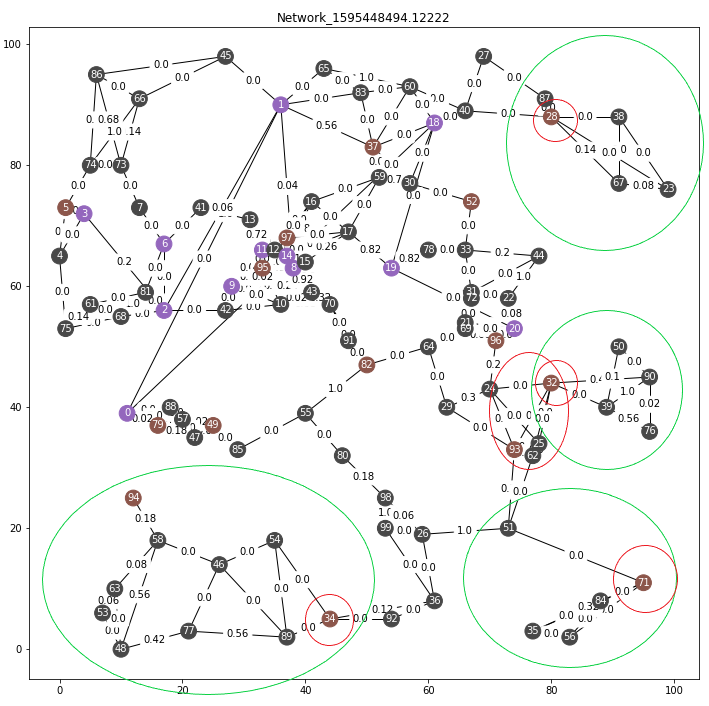
\includegraphics[width=.8\linewidth]{week_3/04 - Component Issues.png}
\caption{The \glspl{component} (circled green) have a \gls{ps} node (circled red), but that node is the \gls{boundary}, so there is no reason the rest of that component would ever be traversed.}
\end{figure}

\begin{itemize}
	\item Added versioning to graphs, so multiple versions of the same graph can be compared.
	\item Made various improvements to increase graph readability and interpretability:
	\begin{itemize}
		\item Increased font size.
		\item Changed \gls{ps} nodes to blue.
		\item Thickened edges and added banded colors along paths between \gls{ps} nodes, so that you can see where they diverge.
		\item Added ability to specify the paths to highlight.
		\item Removed edge labels.
	\end{itemize}
\end{itemize}

\begin{figure}[!ht]
\centering
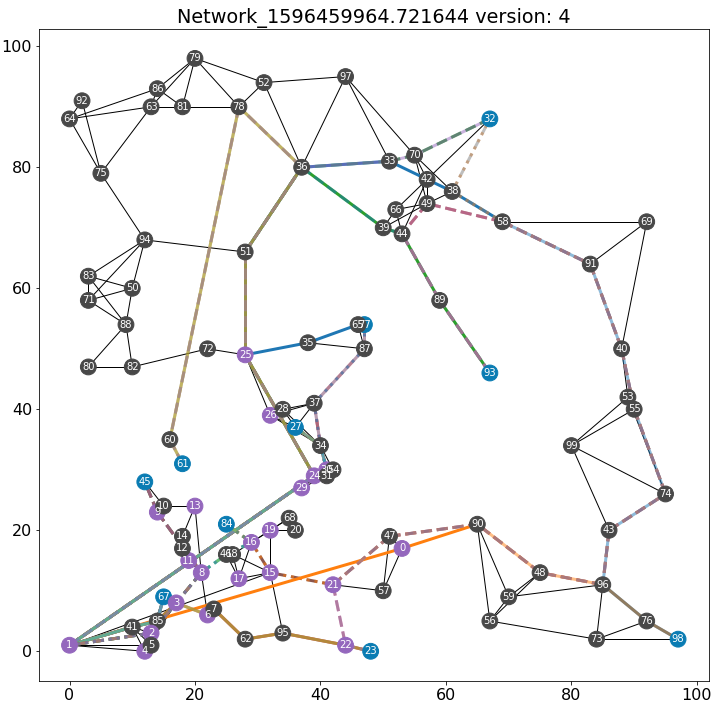
\includegraphics[width=.8\linewidth]{final/color.png}
\caption{Making graphs more readable was helpful in providing a means of visually validating results and troubleshooting as we worked on \gls{tomography}.}
\end{figure}


\subsection*{Incorporating Real Distributions}

Once we had a functioning toy network, we had to determine whether it was in any way a reasonable representation of the real network. In order to do this, we pulled information about the emergent characteristics of the toy network and the same information from the real network, first via \hyperref[kibana]{Kibana} and then directly using the \texttt{\hyperref[es]{elasticsearch}} client in Python (you can read more about these in ~\nameref{app:tools}).

There were three primary metrics we looked at, which all pertained to the paths between \gls{ps} nodes (because that is the only kind of information we have regarding the real network):

\begin{itemize}
    \item The number of \glspl{hop} (how many nodes were along the path to any given destination from any given source).
    \item The total \gls{latency} (sum of the edge lengths, which, in the toy network, was simply Euclidean distance).
    \item The percent \gls{packetloss} (the product of \gls{packetloss} along each edge of a path).
\end{itemize}

In the real data, the number of routes with any given \gls{packetloss} was heavily skewed toward $0$, with a small spike at $100\%$ (when a route had \gls{packetloss}, it was much more likely to have lost all packets). By contrast, looking at all the \gls{ps} pairs for one toy network, we discovered that we were nearing $100\%$ \gls{packetloss}, because we failed to account for the multiplicative nature of \gls{packetloss}.

\begin{figure}[!ht]
\centering
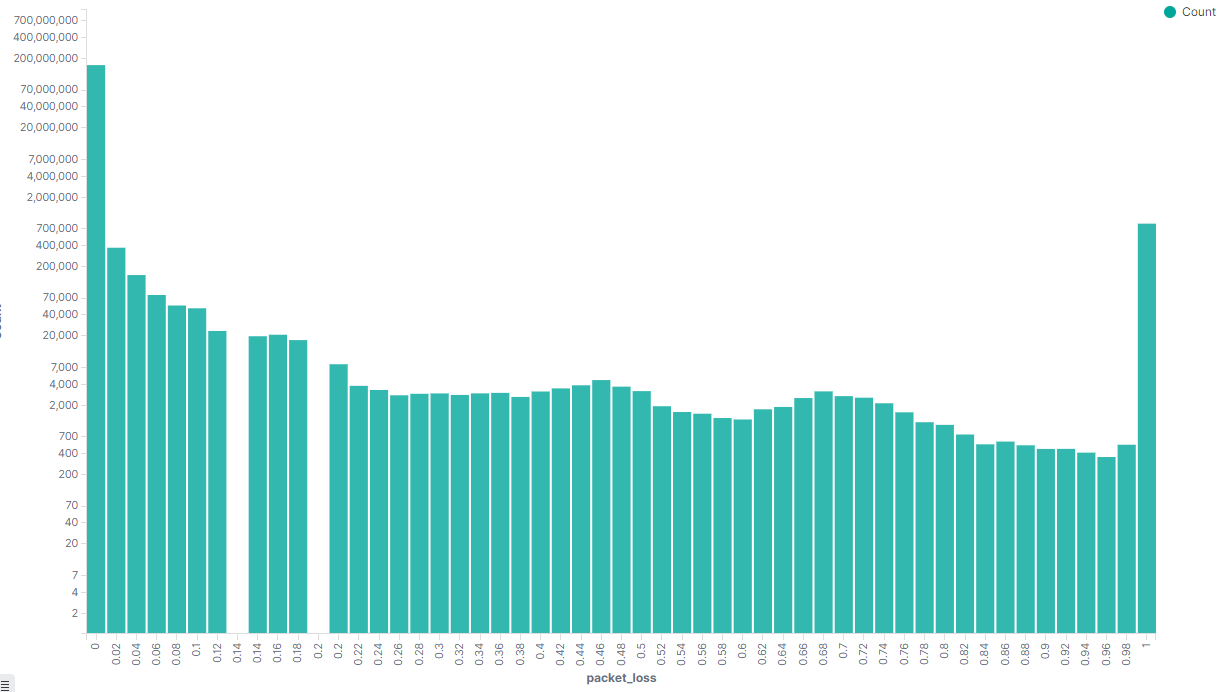
\includegraphics[width=.85\linewidth]{week_2/packetloss.png}
\caption{The count of paths is on a logarithmic scale, so is more heavily skewed than it appears at first glance.}
\end{figure}

\begin{figure}[!ht]
\centering
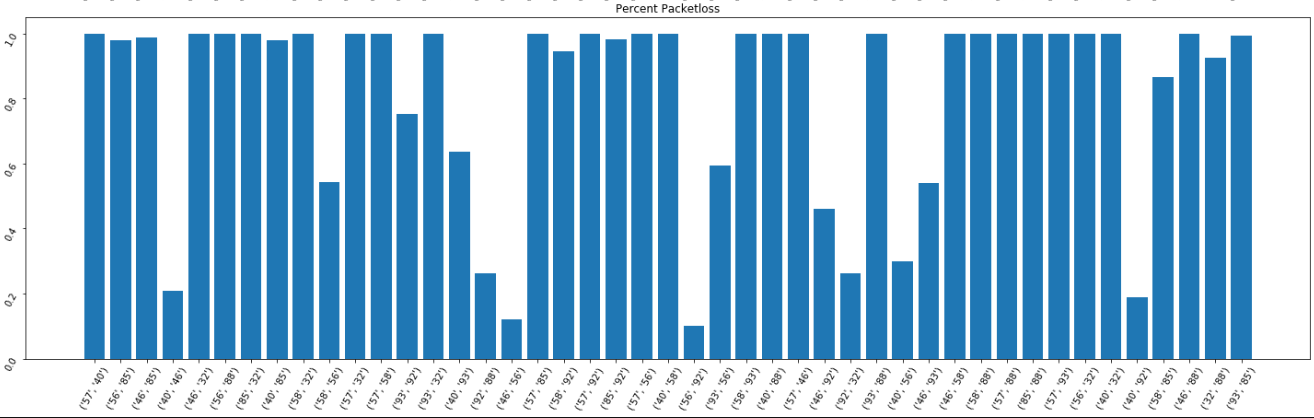
\includegraphics[width=.85\linewidth]{final/toypacketloss.png}
\caption{Most paths in our network were originally approaching $100\%$ \gls{packetloss}.}
\end{figure}

The \gls{latency} in the real network proved problematic, as there were paths with negative latency, a peak near $0$ latency and what looked exponential decay thereafter. It should be impossible to have even $0$ latency, as there is inherently some delay in communicating information over any distance, so this data was clearly erroneous and likely a consequence of clock sync issues. 

\pagebreak
\begin{figure}[!ht]
\centering
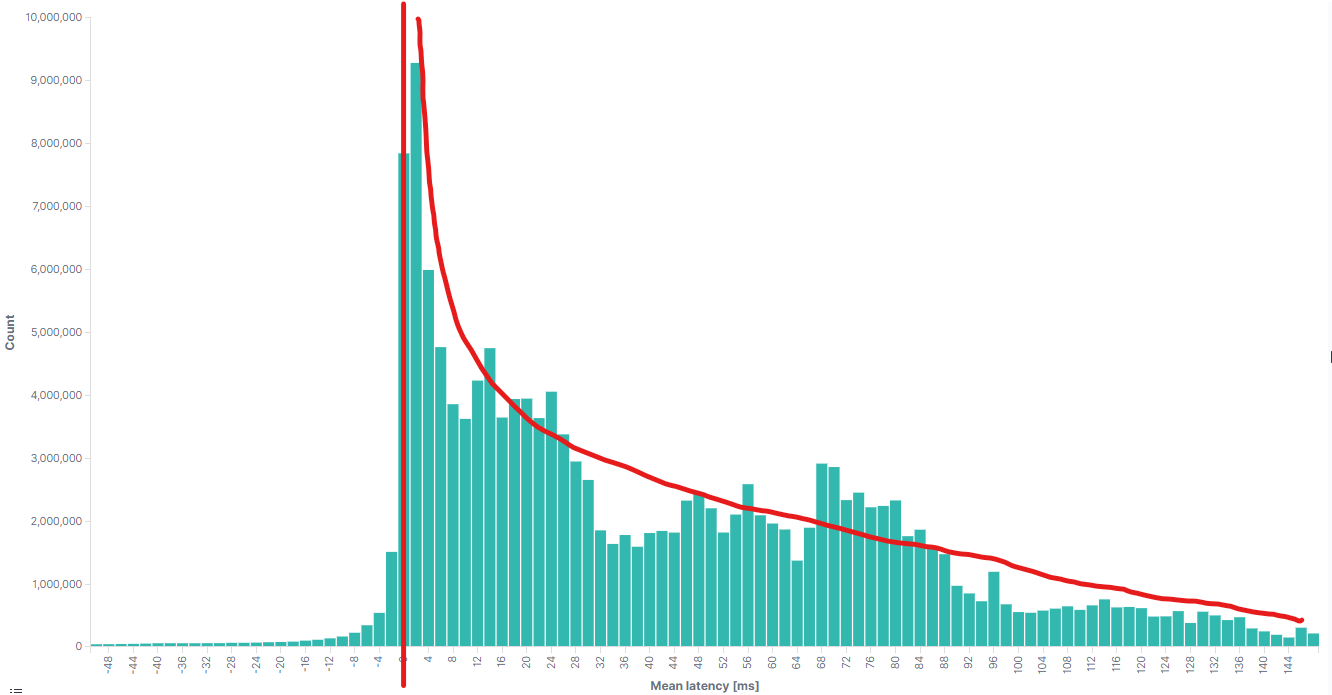
\includegraphics[width=.85\linewidth]{week_4/ExponentialDecay.png}
\caption{The real network had $0$ and negative \glspl{latency}, which is impossible, accompanied by what appeared to be exponential decay.}
\end{figure}

As a stop-gap measure, for want of a better solution, we worked under the (probably incorrect) assumption that all \glspl{latency} were simply offset by roughly $50$ ms. We also took the square root of the counts, to create a better comparison with the scale of the toy network. Though not perfect, we were able to generate some toy networks that roughly resembled this modified distribution.

\begin{figure}[!ht]
\centering
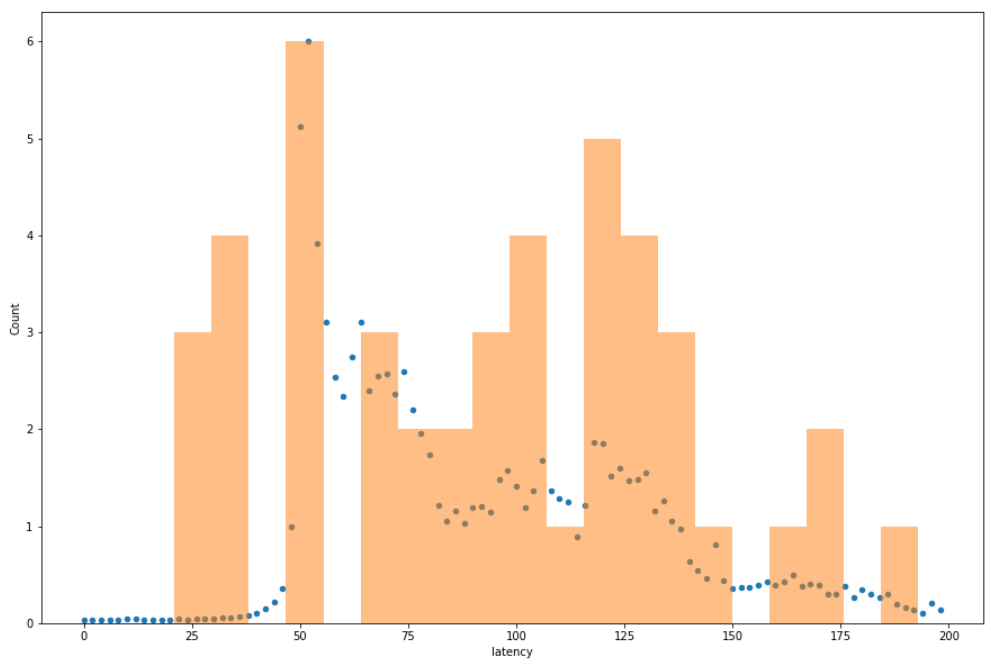
\includegraphics[width=.85\linewidth]{week_4/ToyLatencyHist.png}
\caption{The blue dots represent the square root of the counts of the real network paths with a given \gls{latency}, normalized to a max of 6. The orange histogram represents the count of paths in a given \gls{latency} range.}
\end{figure}


\begin{figure}[!ht]
\centering
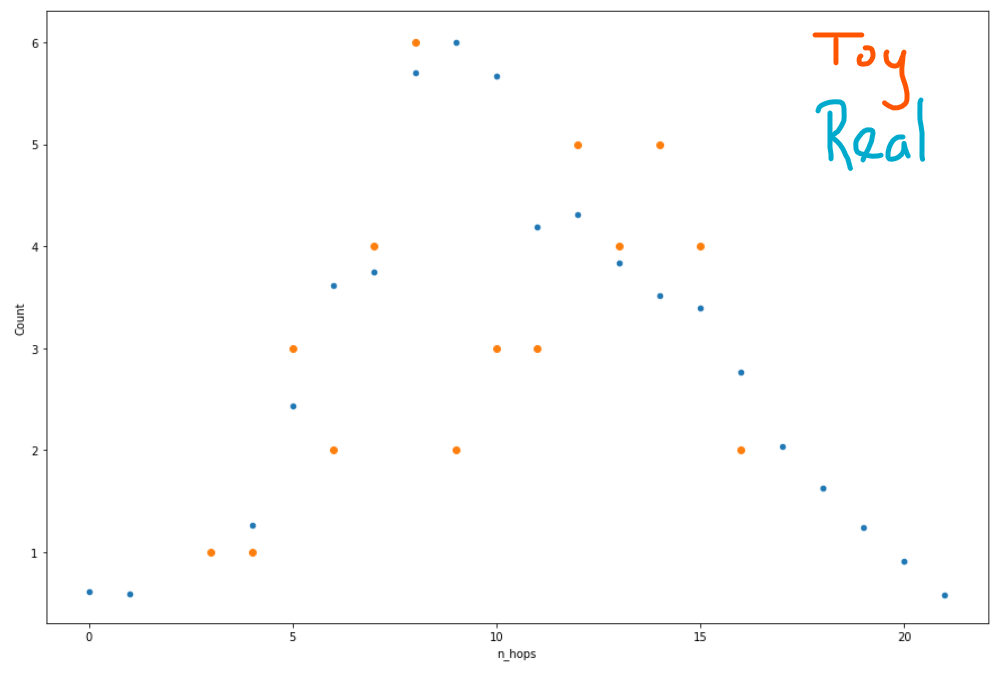
\includegraphics[width=.85\linewidth]{week_4/Hops.png}
\caption{Though the counts required normalization, the average number of \glspl{hop} between \gls{ps} nodes was actually a fairly decent match for what we was emerging from our procedurally generated toy networks.}
\end{figure}

\pagebreak
\section*{Tomography on the Toy Network}

Once I'd built out a fairly robust toy network, that at least somewhat resembled the real one, and the tools to manipulate it (e.g., remove edges, calculate shortest paths, etc.), we were able to manipulate the network, observe changes in network metrics and determine whether it was possible to infer what had been manipulated from those results. The primary case we considered was edge deletion.

\begin{figure}[!ht]
\centering
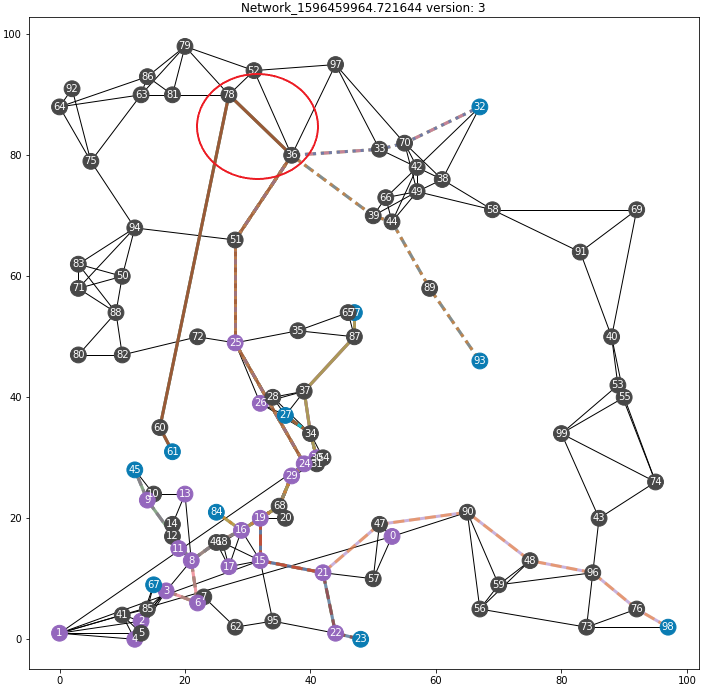
\includegraphics[width=.7\linewidth]{final/OG_78_36.png}
\caption{A toy network, $G$, before any edges have been removed.}
\end{figure}

\noindent We used the following process to determine which edges were deleted:

\begin{enumerate}
	\item Determine the shortest paths between all pairs of \gls{ps} nodes in a toy network, $G$.
	\item Make a copy of that network, $H$.
	\item Delete a single edge in $H$.
	\item Determine the shortest paths between all pairs of \gls{ps} nodes in $H$.
	\item Compare the shortest paths in $H$ to those in $G$:
	\begin{enumerate}
		\item Record edges on each path in $G$ that aren't on the corresponding path in $H$ (i.e., edges that were potentially removed).
		\item Confirm that those edges were entirely removed from $H$ (i.e., they are not on any other paths in $H$).
		\item Determine how many different paths each edge was removed from.
		\begin{itemize}
			\item It's likely that the edge removed from the most paths is the deleted edge.
			\item If multiple edges were removed an equal number of times, there is ambiguity as to which was deleted.
		\end{itemize}
	\end{enumerate}
	\item Repeat 2-5 for each edge in the network.
\end{enumerate}

While experimenting with this process, we also drew the network at each phase and highlighted paths, so that we could see the removed edge and the paths that were rerouted as a result. We plotted the impact of these changes on network metrics like \gls{latency}, \gls{packetloss} and the number of \glspl{hop} on paths. 

\Gls{latency} necessarily increased, as we determined shortest path based on latency, so an edge removed from that path could not be replaced by one with smaller latency. It was quite possible, however, for the total number of \glspl{hop} or the \gls{packetloss} to go down as a result of moving edges, because in our toy network these were not factors in determining paths.

\begin{figure}[!ht]
\centering
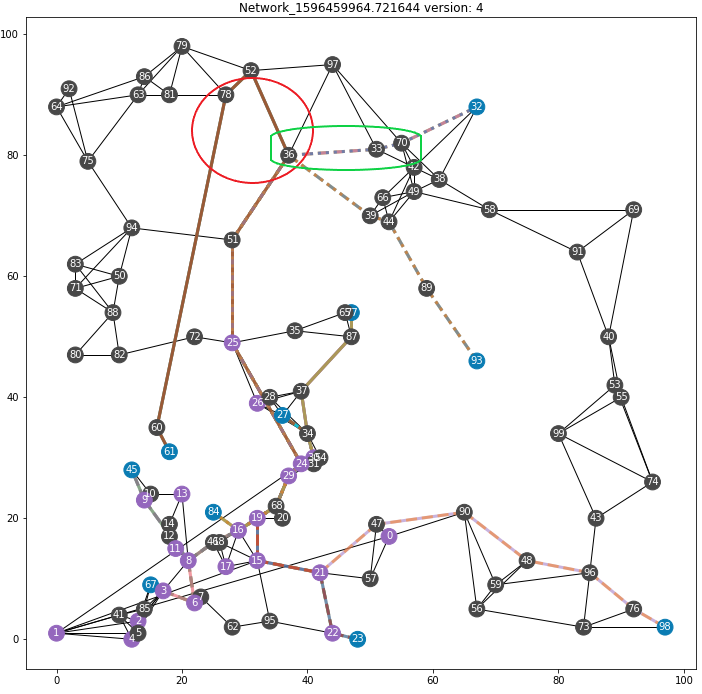
\includegraphics[width=.7\linewidth]{final/New_78_36.png}
\caption{The toy network, $H$, a copy of $G$ with the edge from $78$ to $36$ removed. Note that $(78, 52)$ and $(52, 36)$ are now on a path and that some paths are still using $(36, 33)$ and $(33, 70)$. The significance of that second point is highlighted in the next figure.}
\end{figure}

\begin{figure}[!ht]
\centering
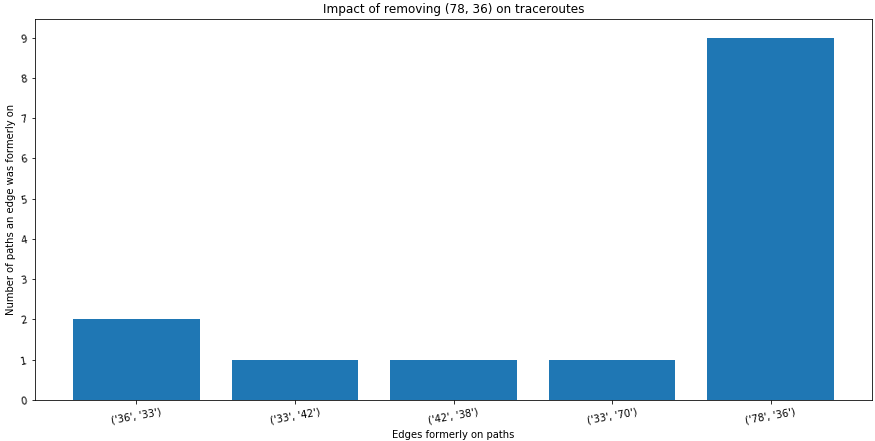
\includegraphics[width=.85\linewidth]{final/Traceroute-78_36.png}
\caption{Only 5 edges were removed from paths as a result of the change. It is pretty clear that $(78, 36)$ is the removed edge, as it was removed from more than 4 times as many routes as any other. Furthermore, we can factor out edges that appear along some other path in $H$, such as $(36, 33)$ and $(33, 70)$.}
\end{figure}

In a real network, a connection between successive \glspl{hop} is rarely completely severed. This strategy would need to be adapted to consider some performance threshold on the real network as being equivalent to an edge being deleted in the toy model.

\section{Modelling the Real Network}

In order to begin applying the lessons learned from the toy network to the real one, we first needed a comparable representation of the real network or some part of it. The data aggregated by real \gls{ps} nodes are indexed several different ways in \hyperref[es]{ElasticSearch} to make it easier to track different characteristics. The two indices we were particularly concerned with were \texttt{trace\_derived\_v2}, which has summative data about all paths in the network over the entirety of our records, and \texttt{ps\_trace}, home of the individual \gls{trace} records the former is derived from.

From the aggregated data in \texttt{trace\_derived\_v2}, we were able to get a list of all \gls{ps} nodes that have served as a source or a destination. Originally, we looked to whittle down these pairs to form a list of paths to look for in the \texttt{ps\_trace} data. For example, we removed ones that had an average number of hops that was less than $1$ (unlike clock sync, we can't really come up with a reason why this would even be recorded as such, but it is clearly impossible to get from one endpoint to another without taking any hops).

We ultimately scrapped the approach of excluding routes based on particular criteria in favor of collecting data on all routes over a given time period and building a core network from that. Having collected $7$ days worth of \texttt{ps\_trace} data, we looked at how long, on average, the path between pairs of \gls{ps} nodes stayed stable. 

The results were encouraging, as the majority of paths lasted the entire $168$ hours without changing even once. When counting pairs of \gls{ps} nodes that had shorter average path lives, the number of paths dropped precipitously as the life of path decreased.

\begin{figure}[!ht]
\centering
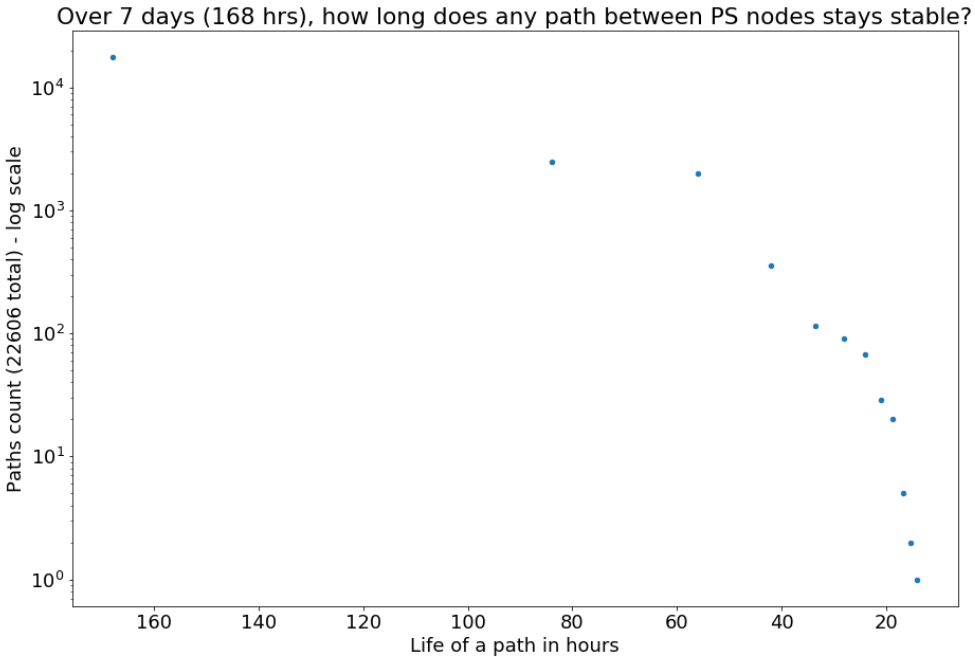
\includegraphics[width=.85\linewidth]{final/pathlife.png}
\caption{Most of the $22,606$ pairs of \gls{ps} nodes had a path that remained stable through the entire $7$ days of data (from $7/7/20-7/14/20$).}
\end{figure}

After determining that most routes are fairly stable, we determined what edges were most central to the network, as follows:

\begin{enumerate}
	\item We created a list of all unique routes and their frequency.
	\item We created a list of edges on each route, by combining all pairs of adjacent \glspl{hop}.
	\item For each edge, we made a weighted sum of the number of unique routes it occurred on (weighted by the frequency of that route's occurrence).
	\item We ordered put this list of edges in reverse order by count, to get a list of edges from the most frequent (a measure of centrality) to the least frequent.
\end{enumerate}

After creating a list of the most frequent edges, we took two different approaches to visualizing them. For both we used the \href{https://networkx.github.io/documentation/stable/reference/generated/networkx.drawing.layout.spring_layout.html}{spring layout} provided by the \hyperref[nx]{\texttt{networkx}} module, but in the first case we graphed only the $n$ most frequent edges, without creating a complete graph of the network. The results showed that the most central edges did tend to be connected, but that there were smaller high frequency clusters of edges that were presumably within a particular region (e.g., the \gls{ps} nodes in the UK are all configured to send messages to each other more frequently than to other nodes on the network).

\begin{figure}[!ht]
\centering
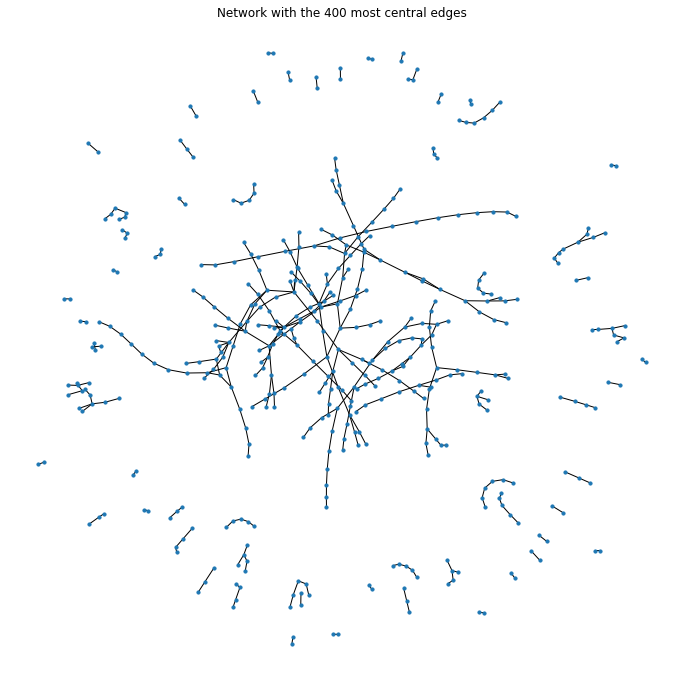
\includegraphics[width=.48\linewidth]{final/n00400.png}
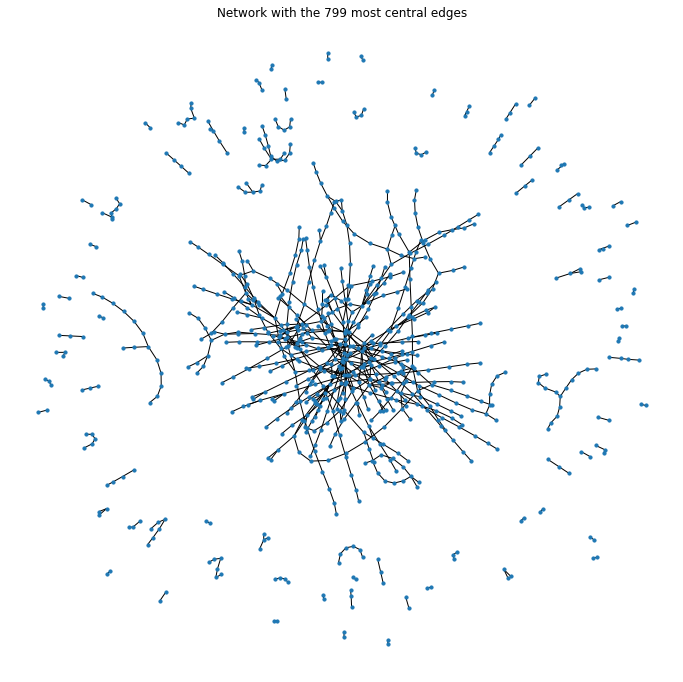
\includegraphics[width=.48\linewidth]{final/n00800.png}
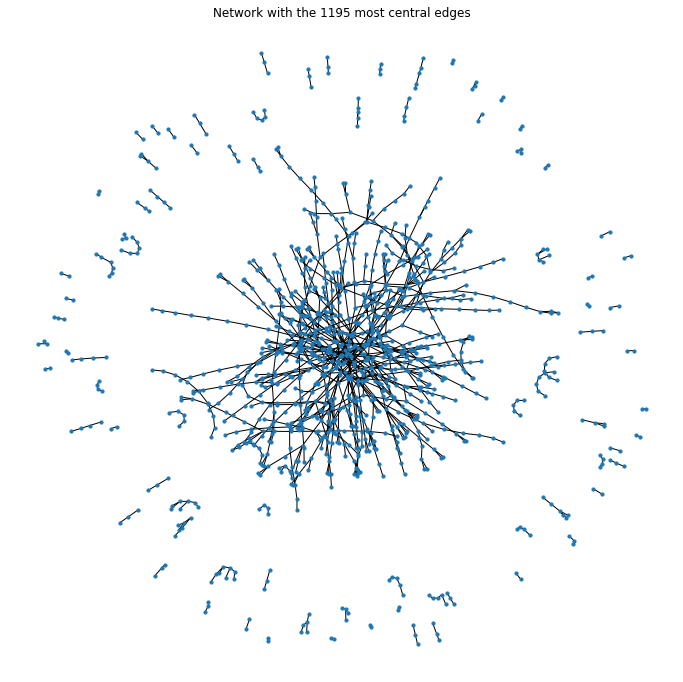
\includegraphics[width=.48\linewidth]{final/n01200.png}
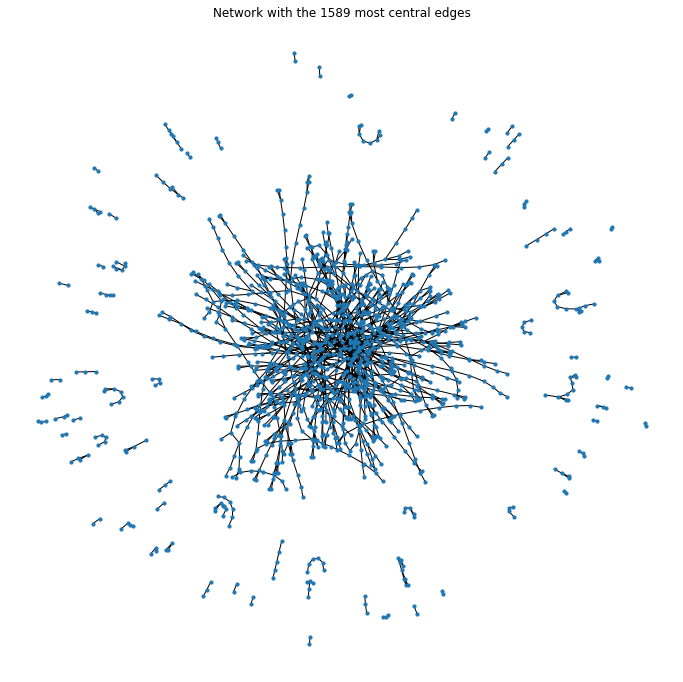
\includegraphics[width=.48\linewidth]{final/n01600.png}
\caption{Redrawing the network with the $400$ most central edges, the $800$ most central and so on, shows that there are clearly clusters of central edges and ones on the periphery probably represent more localized networks.}
\end{figure}

This activity on the periphery eventually decreased (i.e., the clusters became connected to the larger network) as we increased the how many of the most frequent edges we considered. While this was expected, we also began to note a less expected phenomena. 

The number of most central edges actually being plotted was not quite tracking with the number of edges being supplied. The deviance increased/became more apparent as the number of edges to be plotted increased. Upon investigation the reason for this appeared to be symmetric edges, which were being supplied twice (e.g., once as $(a, b)$ and once as $(b, a)$), but only graphed once. We would have expected this to be a very common occurrence, but, upon further investigation, only about $2\%$ of edges were symmetric.

\begin{figure}[!ht]
\centering
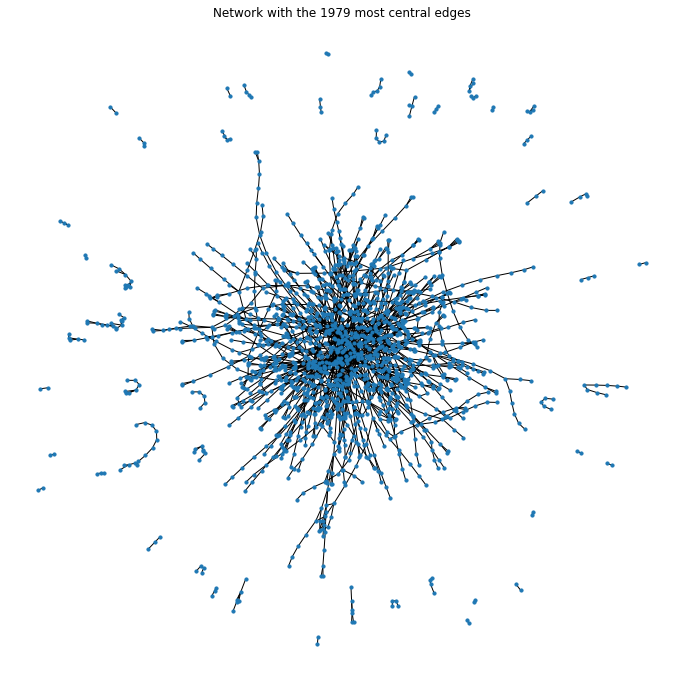
\includegraphics[width=.46\linewidth]{final/n02000.png}
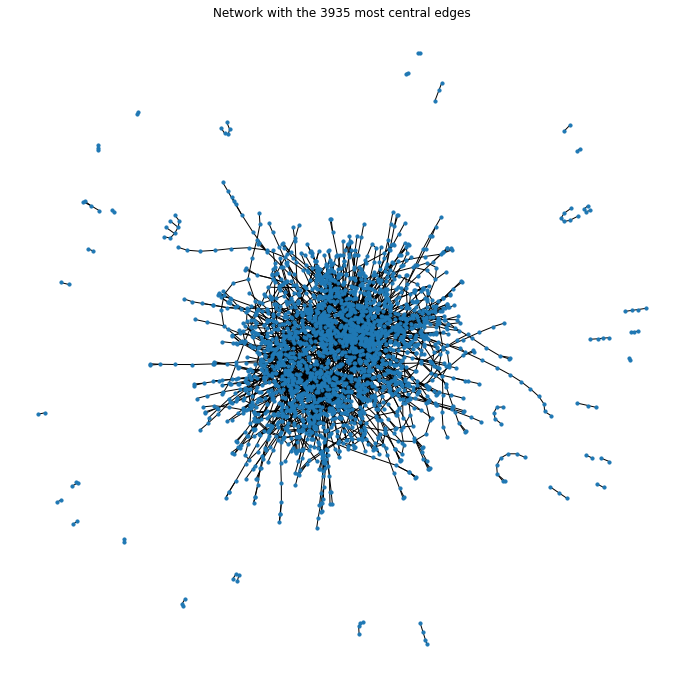
\includegraphics[width=.46\linewidth]{final/n04000.png}
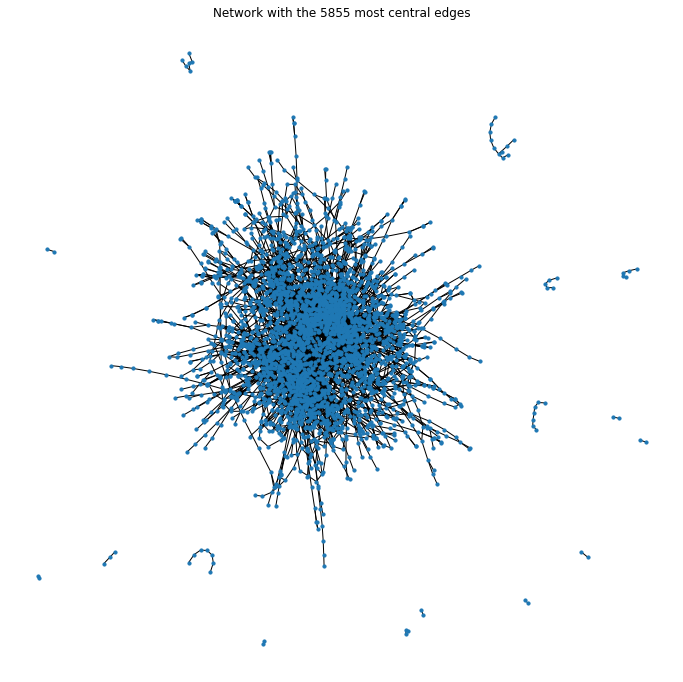
\includegraphics[width=.46\linewidth]{final/n06000.png}
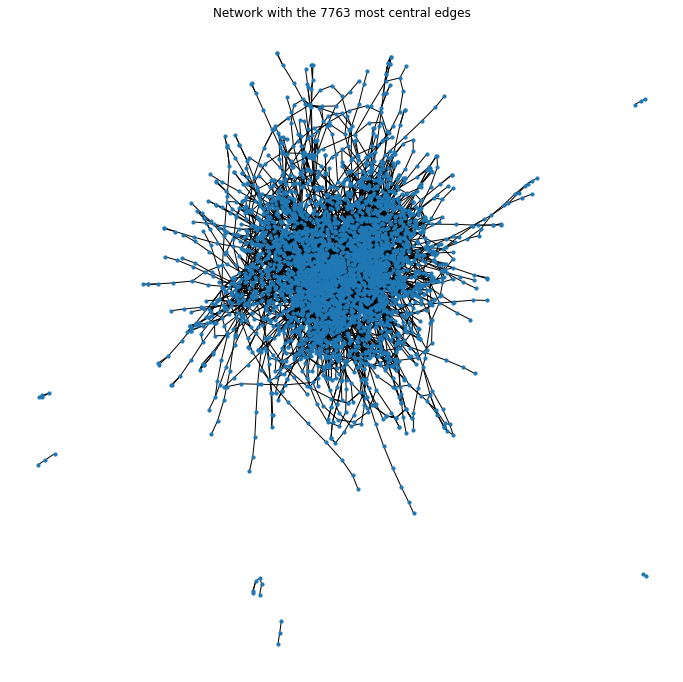
\includegraphics[width=.46\linewidth]{final/n08000.png}
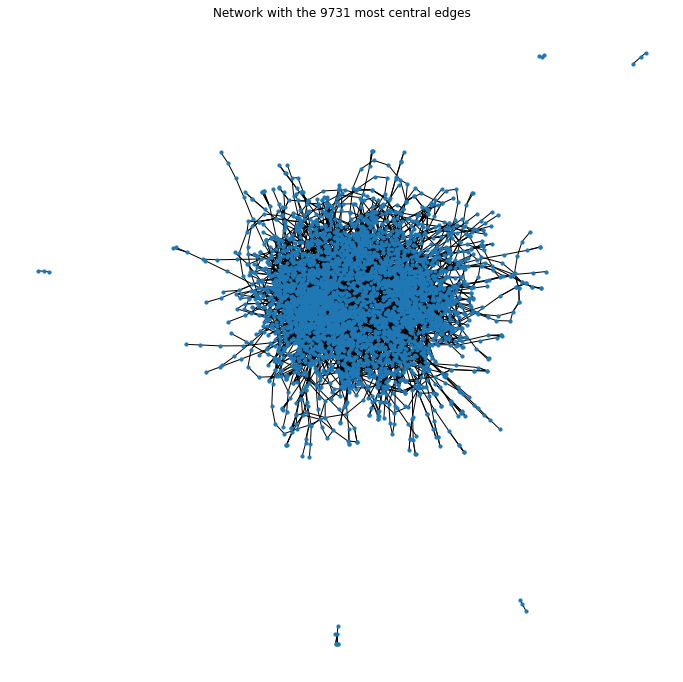
\includegraphics[width=.46\linewidth]{final/n10000.png}
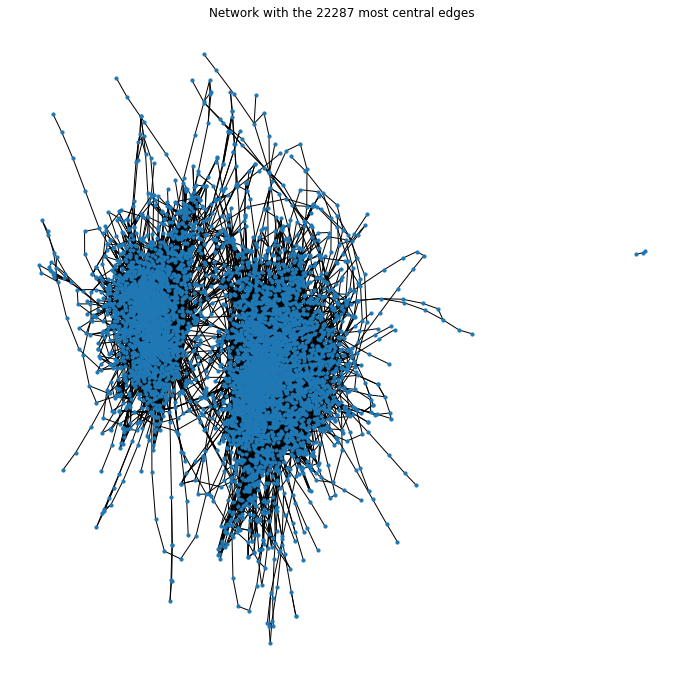
\includegraphics[width=.46\linewidth]{final/n22817.png}
\caption{As the number of edges increased, the number of edges that remained unconnected decreased.}
\end{figure}

There was some interesting phenomena once we finally reached a complete graphing of the network, namely, the graph clearly split into two distinct clusters. This presumably represents the continental divide, but what was interesting about this is that the edges splitting the clusters were not of high enough frequency that the clusters became distinct early on. 

To get an idea of how the network builds up as we increase the number of edges, it seemed prudent to repeat the process, but having fixed the entire graph layout before drawing any edges. This meant keeping the relative positions of all the nodes constant, but only drawing those incident to the $n$ most frequent edges.

\begin{figure}[!ht]
\centering
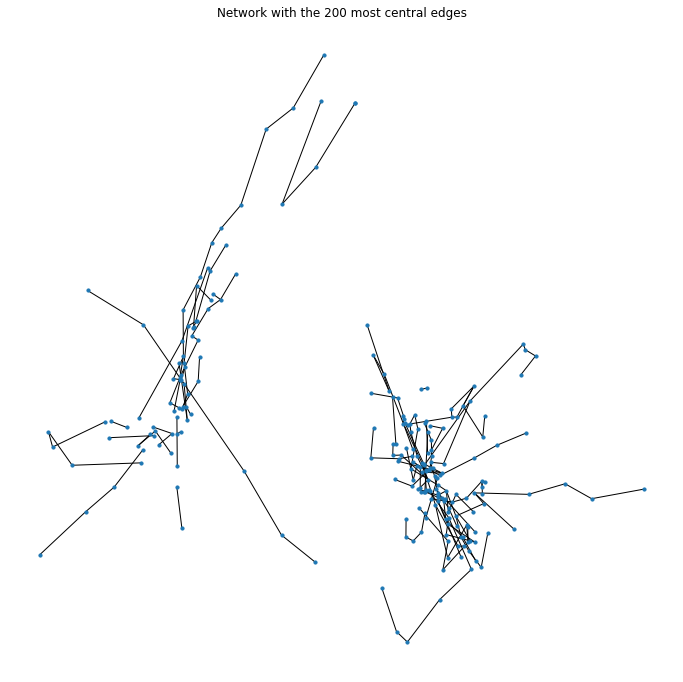
\includegraphics[width=.48\linewidth]{final/f00200.png}
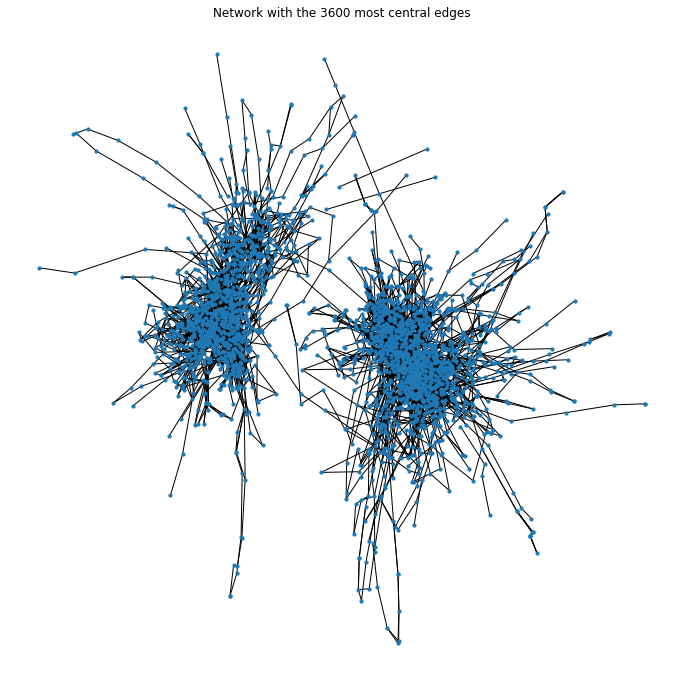
\includegraphics[width=.48\linewidth]{final/f03600.png}
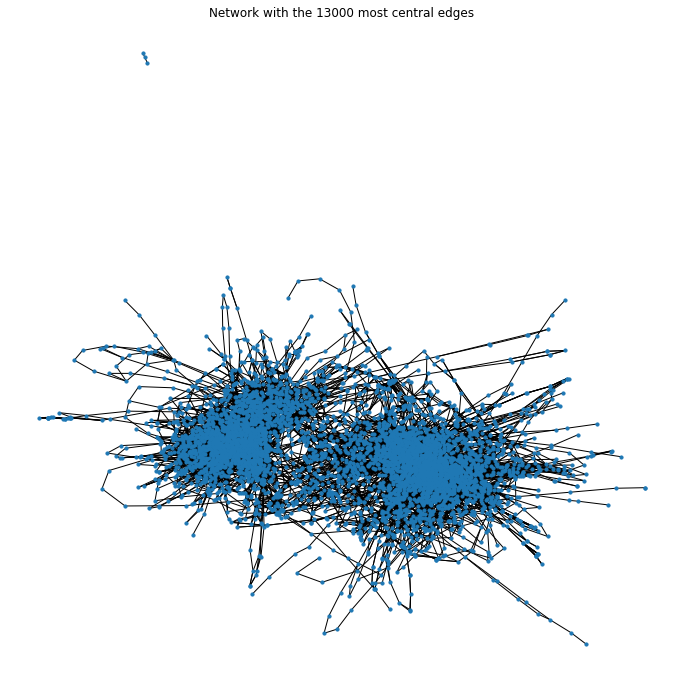
\includegraphics[width=.48\linewidth]{final/f13000.png}
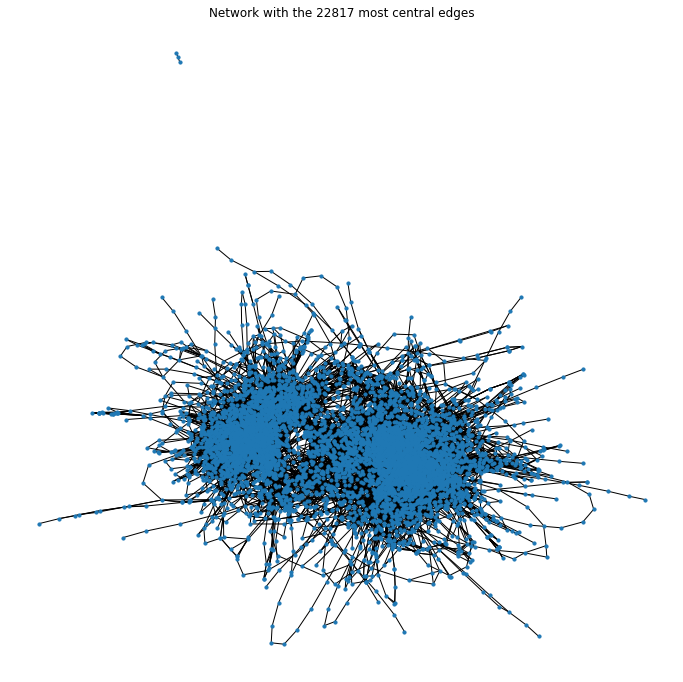
\includegraphics[width=.48\linewidth]{final/f22817.png}
\caption{The continental divide is more apparent when graphing edges in the context of their position in a spring layout for the entire network.}
\end{figure}

It appears that the majority of \gls{ps} nodes are in most frequent communication with other nodes that are in the same region (as opposed to ones on the other side of the Atlantic), which explains why that divide is not apparent until very late when graphing without the context of the entire network. 

\pagebreak
\section*{Topics for Further Study}

With the determination of which edges are most frequent and the ability to construct graphs of the real network in the same fashion we did graphs of the toy network, the door is open to further investigation and transference of lessons learned on the toy network to use with the real network. Below is a brief list of just a few outstanding questions/topics that would be worth exploring further:

\begin{itemize}
	\item How significant is the impact of the asymmetry of edges on the network?
	\item Are there ways to account for this asymmetry?
	\item Similarly, there may be multiple representations of the same devices and \gls{ps} nodes on the network, most notably IPv4 vs. IPv6 identifiers; can we map different representations of a device to the same device?
	\item Knowing that certain edges are very central to the network, can we monitor those specific edges for potential performance issues, to allow us to identify network issues sooner?
	\item Alternatively, could we use \gls{anomaly} to identify when to investigate some portion of the network?
	\item Would the same strategy used with the toy network (determining edges that were removed from multiple impacted paths), allow us to pinpoint issues on the real network?
\end{itemize}

\section{Summary}

\section{Acknowledgments}

\pagebreak

\printbibheading
\printbibliography[keyword=major,heading=subbibliography,title={Primary Sources}]
\printbibliography[keyword=minor,heading=subbibliography,title={Further Reading}]

\section{Appendix A: Terms}\label{app:gloss}

\printnoidxglossaries

\section{Appendix B: Tools Used}\label{app:tools}

\subsection{Describing the network: \texttt{networkx}}\label{nx}

For creating an underlying representation of the network, we used the \texttt{networkx}\cite{nx} package in Python. This provided a graph object with various means of adding nodes, edges and metadata. It also provided tools for determining graph characteristics, such as bridge-connected components\cite{nxb}, $k$-connectivity\cite{nxk} and betweeness centrality\cite{nxc}.

\subsection{Drawing the network and plotting data: \texttt{matplotlib}}\label{mpl}

For drawing the network, \texttt{networkx}\cite{nx} integrates with \texttt{matplotlib}\cite{mpl}. This gave me a means of specifying (or not) the locations of nodes, as well as drawing, labeling and coloring specific nodes and edges.

We also used \texttt{matplotlib} in conjunction with \texttt{NumPy}\cite{np} arrays and \texttt{pandas}\cite{pd} dataframes in order to create various charts and histograms.

\subsection{Exploring real network data: Kibana}\label{kibana}

For preliminary data exploration, we used Kibana\cite{kibana}, which provided visualizations such as histograms and tables. It also provided, via the Console and the Inspect tool (available on all visualizations), a means of testing and exploring how ElasticSearch's Query DSL\cite{query} works.

\subsection{Querying real network data: ElasticSearch Query DSL}\label{es}

For pulling large amounts of data for analysis, we used the \texttt{elasticsearch}\cite{es} client in Python, which provides an API for ElasticSearch's Query DSL\cite{query}. More specifically, for small queries we used \texttt{search} which can provide only limited results. For larger amounts of data, we used \texttt{scan}, which is a helper for the \texttt{bulk} API.

\end{document}